\hypertarget{mtk_8h}{\section{include/mtk.h File Reference}
\label{mtk_8h}\index{include/mtk.\+h@{include/mtk.\+h}}
}


Includes the entire A\+P\+I.  


{\ttfamily \#include \char`\"{}mtk\+\_\+roots.\+h\char`\"{}}\\*
{\ttfamily \#include \char`\"{}mtk\+\_\+enums.\+h\char`\"{}}\\*
{\ttfamily \#include \char`\"{}mtk\+\_\+tools.\+h\char`\"{}}\\*
{\ttfamily \#include \char`\"{}mtk\+\_\+matrix.\+h\char`\"{}}\\*
{\ttfamily \#include \char`\"{}mtk\+\_\+dense\+\_\+matrix.\+h\char`\"{}}\\*
{\ttfamily \#include \char`\"{}mtk\+\_\+blas\+\_\+adapter.\+h\char`\"{}}\\*
{\ttfamily \#include \char`\"{}mtk\+\_\+lapack\+\_\+adapter.\+h\char`\"{}}\\*
{\ttfamily \#include \char`\"{}mtk\+\_\+glpk\+\_\+adapter.\+h\char`\"{}}\\*
{\ttfamily \#include \char`\"{}mtk\+\_\+uni\+\_\+stg\+\_\+grid\+\_\+1d.\+h\char`\"{}}\\*
{\ttfamily \#include \char`\"{}mtk\+\_\+uni\+\_\+stg\+\_\+grid\+\_\+2d.\+h\char`\"{}}\\*
{\ttfamily \#include \char`\"{}mtk\+\_\+uni\+\_\+stg\+\_\+grid\+\_\+3d.\+h\char`\"{}}\\*
{\ttfamily \#include \char`\"{}mtk\+\_\+grad\+\_\+1d.\+h\char`\"{}}\\*
{\ttfamily \#include \char`\"{}mtk\+\_\+div\+\_\+1d.\+h\char`\"{}}\\*
{\ttfamily \#include \char`\"{}mtk\+\_\+lap\+\_\+1d.\+h\char`\"{}}\\*
{\ttfamily \#include \char`\"{}mtk\+\_\+robin\+\_\+bc\+\_\+descriptor\+\_\+1d.\+h\char`\"{}}\\*
{\ttfamily \#include \char`\"{}mtk\+\_\+quad\+\_\+1d.\+h\char`\"{}}\\*
{\ttfamily \#include \char`\"{}mtk\+\_\+interp\+\_\+1d.\+h\char`\"{}}\\*
{\ttfamily \#include \char`\"{}mtk\+\_\+grad\+\_\+2d.\+h\char`\"{}}\\*
{\ttfamily \#include \char`\"{}mtk\+\_\+div\+\_\+2d.\+h\char`\"{}}\\*
{\ttfamily \#include \char`\"{}mtk\+\_\+curl\+\_\+2d.\+h\char`\"{}}\\*
{\ttfamily \#include \char`\"{}mtk\+\_\+lap\+\_\+2d.\+h\char`\"{}}\\*
{\ttfamily \#include \char`\"{}mtk\+\_\+robin\+\_\+bc\+\_\+descriptor\+\_\+2d.\+h\char`\"{}}\\*
{\ttfamily \#include \char`\"{}mtk\+\_\+grad\+\_\+3d.\+h\char`\"{}}\\*
{\ttfamily \#include \char`\"{}mtk\+\_\+div\+\_\+3d.\+h\char`\"{}}\\*
{\ttfamily \#include \char`\"{}mtk\+\_\+lap\+\_\+3d.\+h\char`\"{}}\\*
{\ttfamily \#include \char`\"{}mtk\+\_\+robin\+\_\+bc\+\_\+descriptor\+\_\+3d.\+h\char`\"{}}\\*
{\ttfamily \#include \char`\"{}mtk\+\_\+operator\+\_\+applicator.\+h\char`\"{}}\\*
Include dependency graph for mtk.\+h\+:
\nopagebreak
\begin{figure}[H]
\begin{center}
\leavevmode
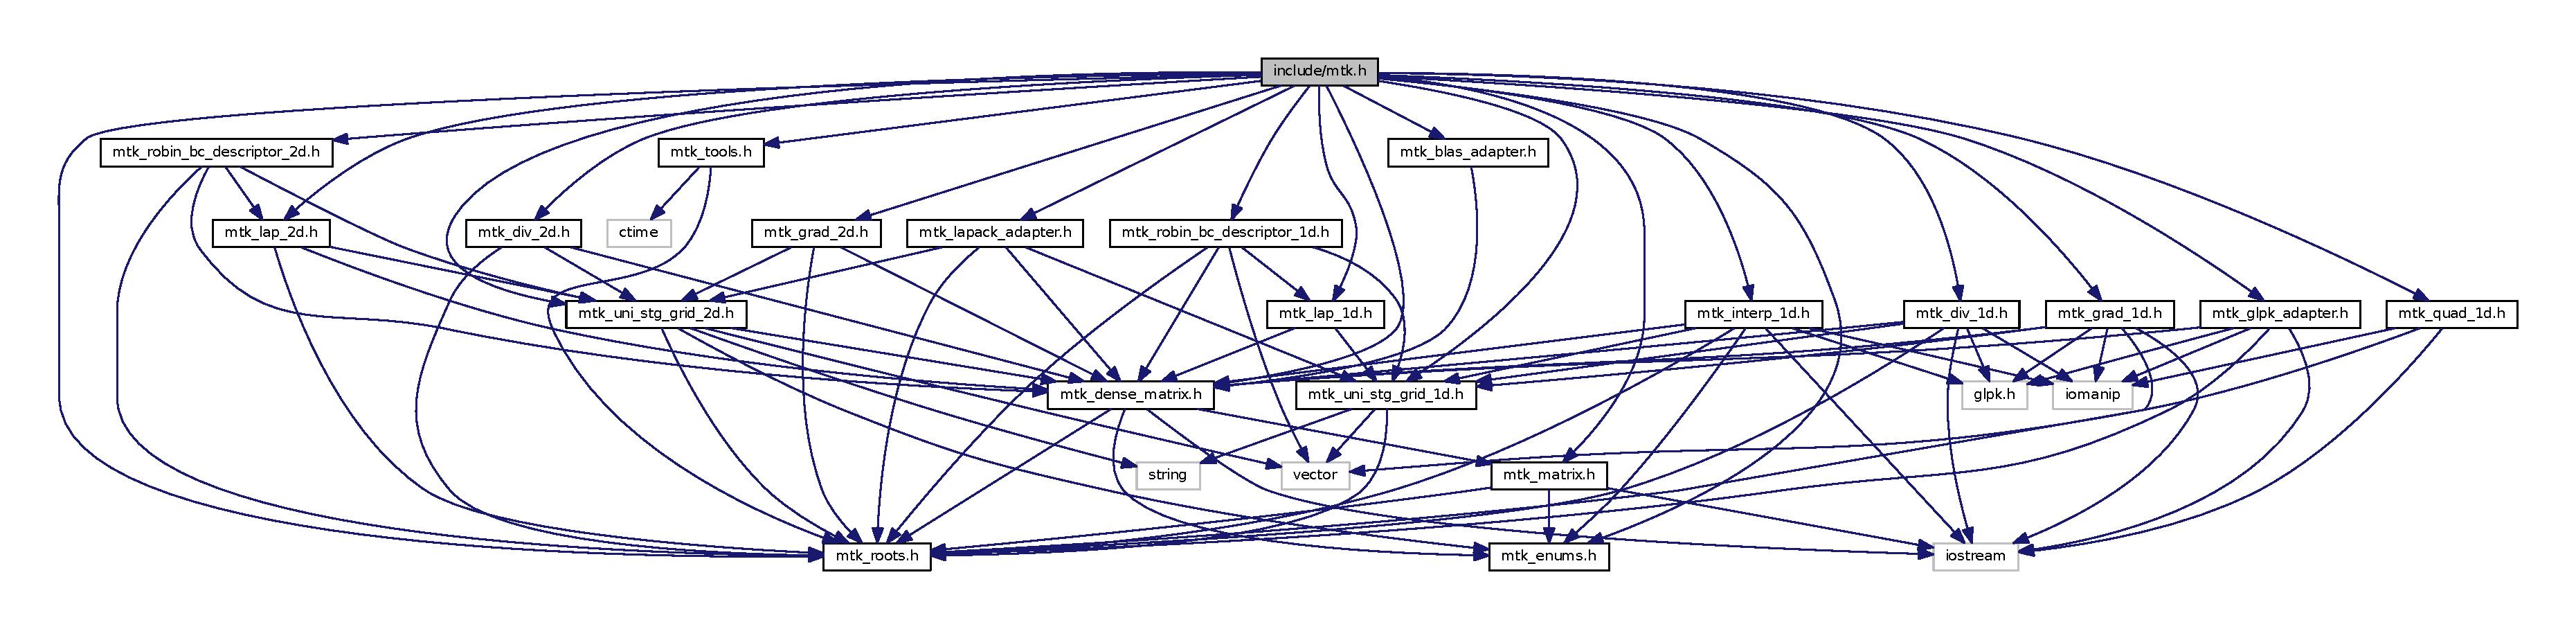
\includegraphics[width=350pt]{mtk_8h__incl}
\end{center}
\end{figure}


\subsection{Detailed Description}
This file contains every required header file, thus containing the entire A\+P\+I. In this way, client codes only have to instruct \#include \char`\"{}mtk.\+h\char`\"{}.

\begin{DoxyWarning}{Warning}
It is extremely important that the headers are added to this file in a specific order; that is, considering the dependence between the classes these contain.
\end{DoxyWarning}
\begin{DoxyAuthor}{Author}
\+: Eduardo J. Sanchez (ejspeiro) -\/ esanchez at mail dot sdsu dot edu 
\end{DoxyAuthor}


Definition in file \hyperlink{mtk_8h_source}{mtk.\+h}.

